%%%%%%%%%%%%%%%%%%%%%%%%%%%%%%%%%%%%%%%%%%%%%%%%%%%%%%%%%%%%%%%%%%%%%%%%%%%%%%%%
% TUM-Vorlage: Präsentation - Beispiele
%%%%%%%%%%%%%%%%%%%%%%%%%%%%%%%%%%%%%%%%%%%%%%%%%%%%%%%%%%%%%%%%%%%%%%%%%%%%%%%%

\begin{frame}
	\frametitle{XSD- tree-like definition of Datastructures}
	\begin{figure}
		\centering
		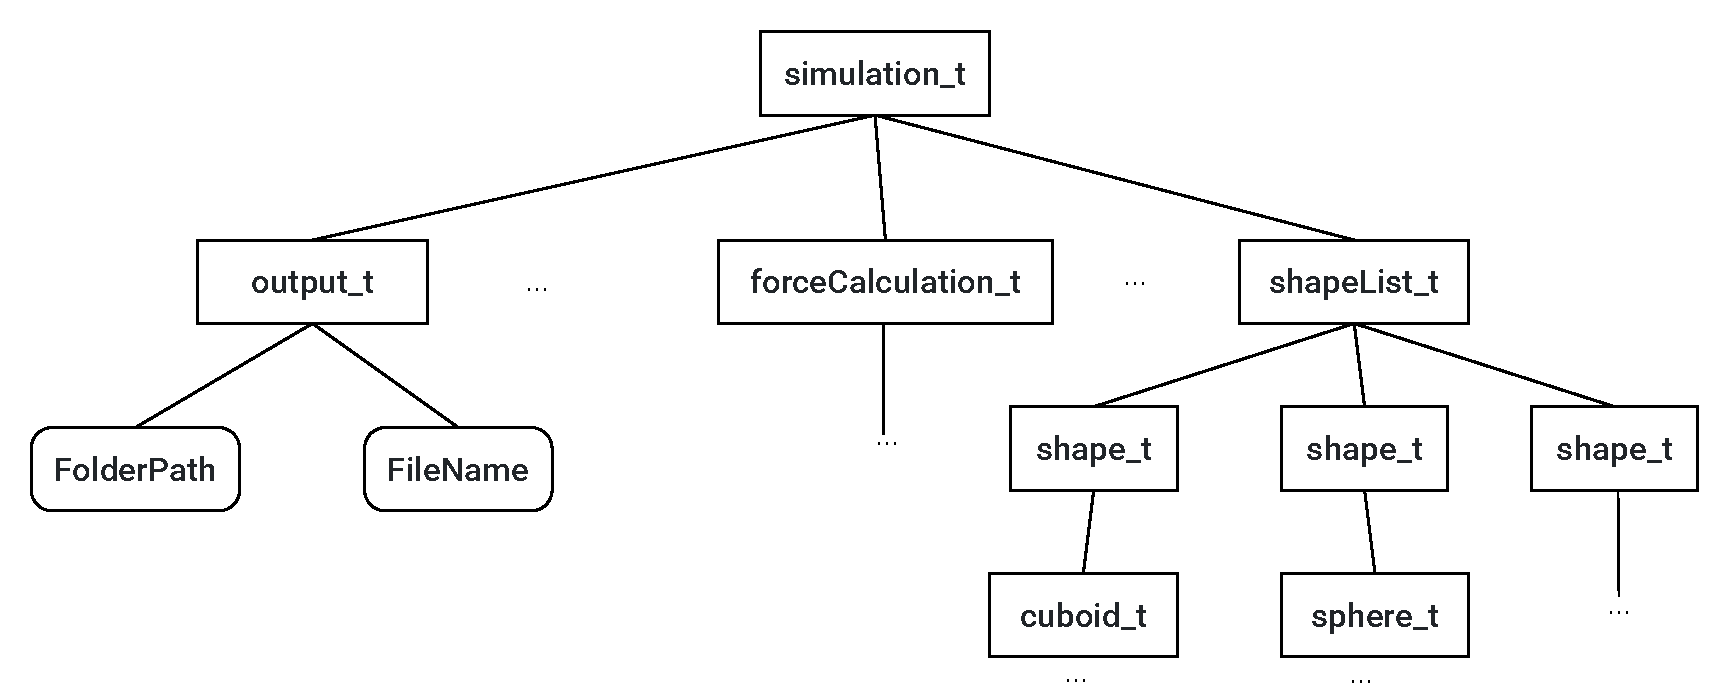
\includegraphics[width=\linewidth]{xsdScetch}
		%\caption{}
		\label{fig:xsdscetchtbc}
	\end{figure}
	
	
\end{frame}

\begin{frame}[fragile]
	\frametitle{XSD- Code Snippet}
	\large
	\begin{itemize}
		\item simulation\_t stores all the necessary parameters
		\item Definition utilizes other Datastructures with tree-like definitions
		\item "'simulation\_t is root"'
	\end{itemize}
	
	\vspace{0.3cm}
	
	\begin{lstlisting}
<xsd:complexType name="simulation_t">
	<xsd:sequence>
		<xsd:element name="OutputFile" type="output_t" minOccurs="0"/>
		...
		<xsd:element name="ShapeList" type="shapeList_t"/>
	</xsd:sequence>
</xsd:complexType>
	\end{lstlisting}
\end{frame}

\begin{frame}[fragile]
	\frametitle{XSD- Code Snippet}
	\Large
	Trade-Off convenience $\leftrightarrow$ complexity in action:
	\large
	\vspace{1cm}
	\begin{lstlisting}
<xsd:complexType name="shape_t">
	<xsd:choice>
		<xsd:element name="Particle" type="particle_t"/>
		<xsd:element name="Cuboid" type="cuboid_t"/>
		<xsd:element name="Sphere" type="sphere_t"/>
	</xsd:choice>
</xsd:complexType>
	\end{lstlisting}
	
\end{frame}


\begin{frame}
	\frametitle{Bounds Handling}
	\large
	\begin{figure}
		\centering
		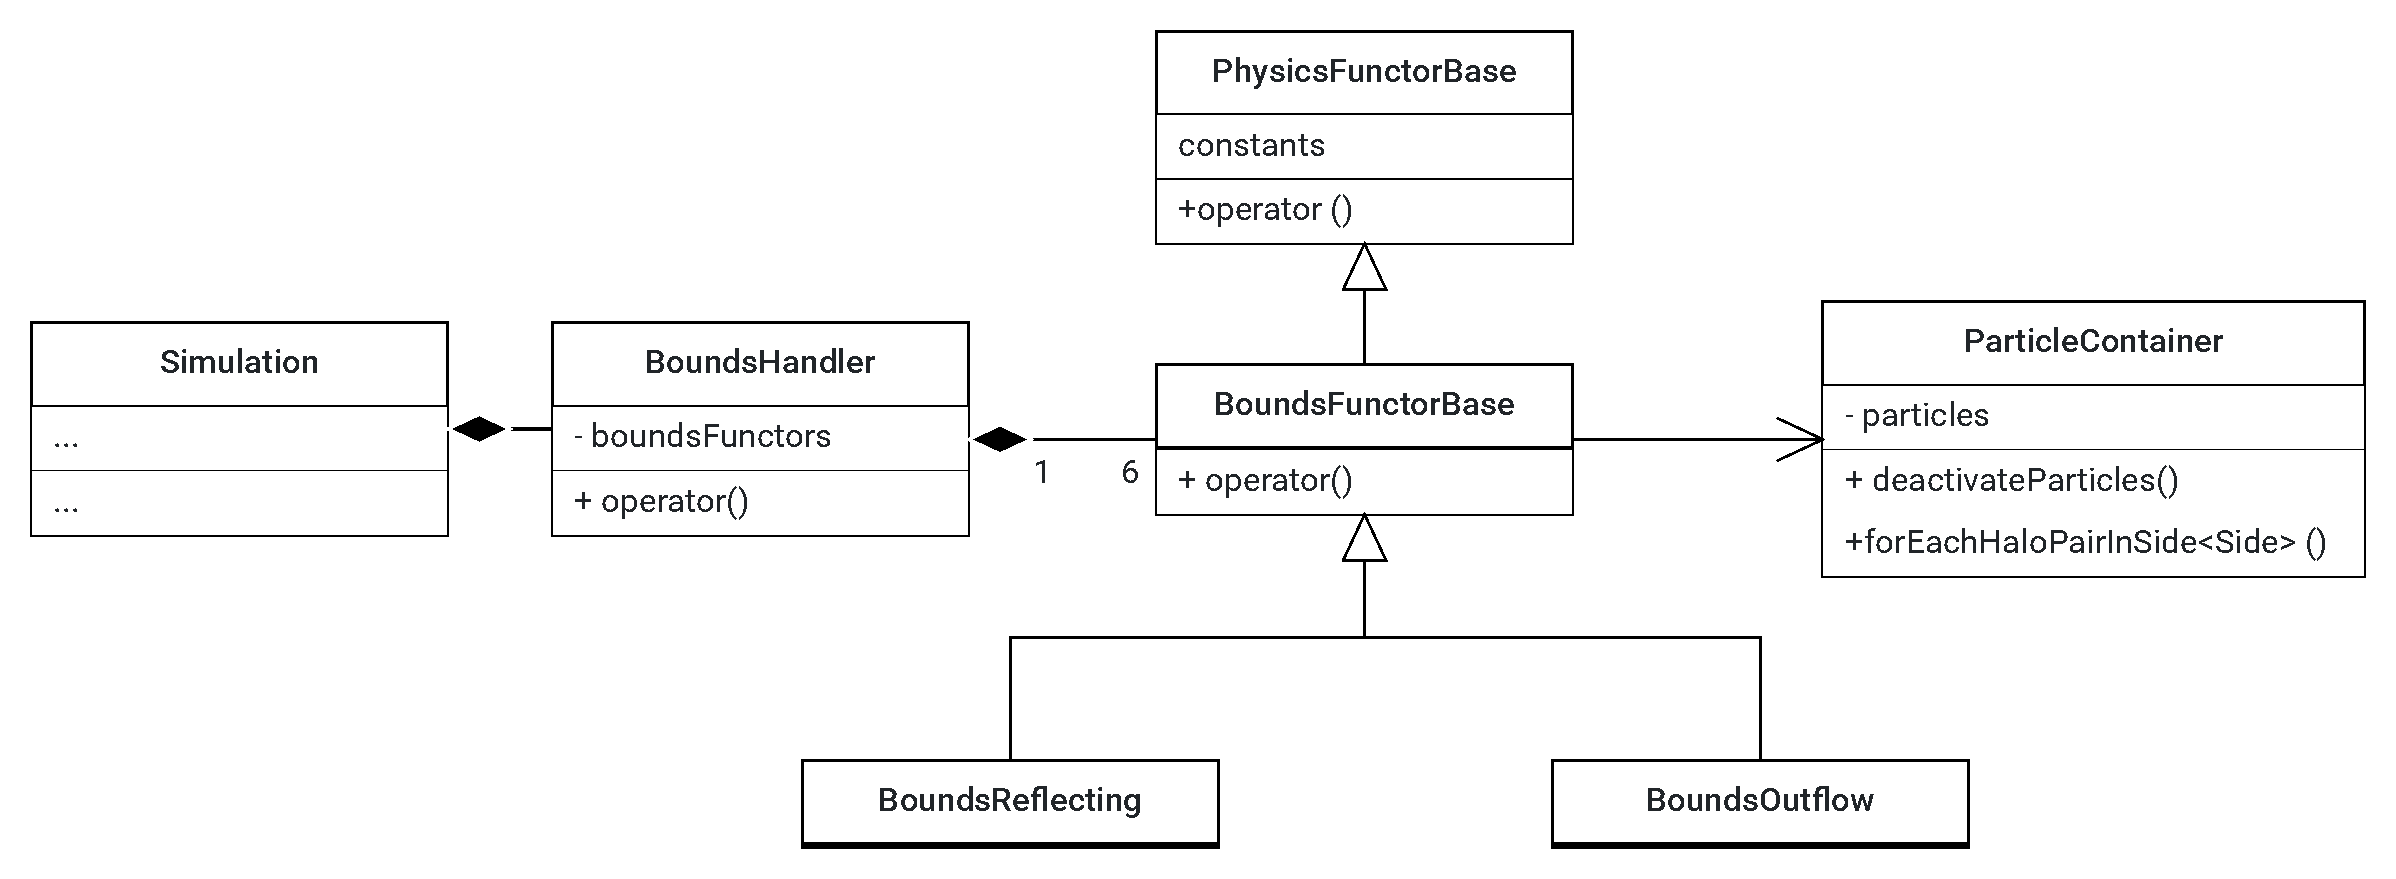
\includegraphics[width=0.9\linewidth]{BoundaryMolSim}
		\label{fig:boundarymolsim}
	\end{figure}
\end{frame}



\begin{frame}
	\frametitle{ForceFunctors}
	\large
	\begin{itemize}
		\item Force function used gets determined on runtime via input parameters
		\item Force functor defines the algorithm (Linked-Cell algorithm/ All-Pairs algorithm) used
	\end{itemize}
	\vspace{-0.4cm}
	
	\begin{figure}
		\centering
		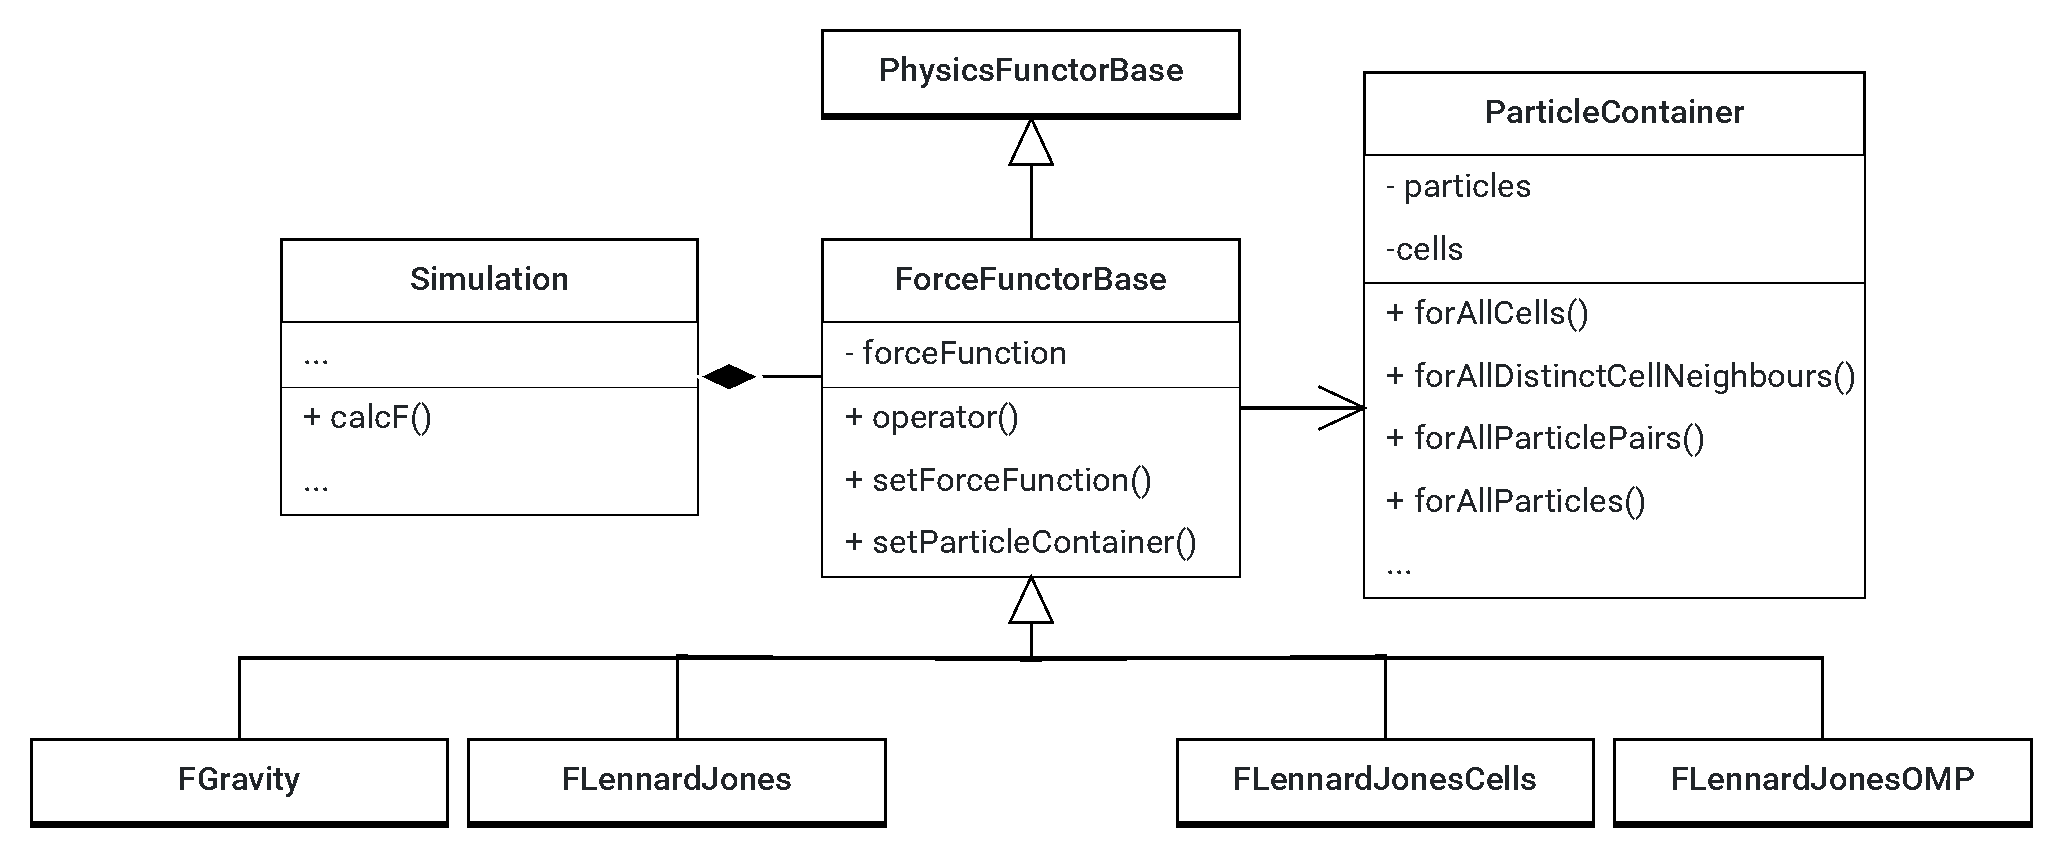
\includegraphics[width=0.8\linewidth]{ForceFunctorMolSim}
		\label{fig:forcefunctormolsim}
	\end{figure}
	
\end{frame}

\begin{frame}[fragile]
	\frametitle{Spheres}
	\large
	Expansion of the Body-struct utilized in Assignment 2
	
	\begin{columns}
		
		\begin{column}{0.48\textwidth}
			\begin{lstlisting}[language=C++]	
enum Shape {cuboid, sphere};
struct Body {
	Shape shape;   
	Eigen::Vector3d fixpoint; 
	Eigen::Vector3d dimensions;
	double distance;
	double mass;
	Eigen::Vector3d start_velocity;
} ;
			\end{lstlisting}	
		\end{column}
		
		\begin{column}{0.48\textwidth}
			\vspace{-1.5cm}
			\begin{equation*}
				\begin{aligned}
					\sqrt{x^2 + y^2 + z^2} & <= r\\
					\iff x^2 + y^2 + z^z   & <= r^2
				\end{aligned}
			\end{equation*}
			
			\vspace{0.5cm}
			
			\begin{center}
				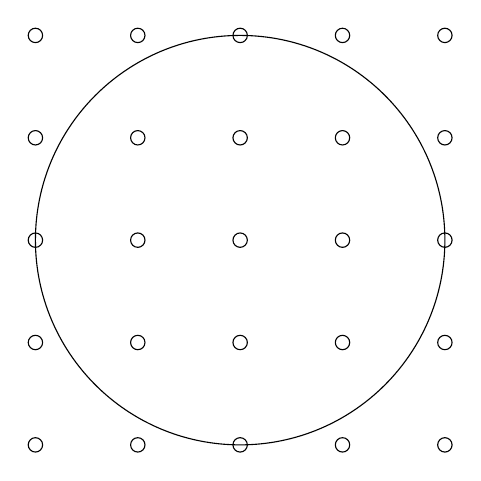
\begin{tikzpicture}[scale=1.3]
					\foreach \x in {0,...,4}{
						\foreach \y in {0,...,4}{
							\draw (\x, \y) circle[radius=2pt];
						}
					}
					
					\draw (2,2) circle[radius=2];
					
					
				\end{tikzpicture}
			\end{center}
		\end{column}
		
	\end{columns}
	
\end{frame}



\begin{frame}
\frametitle{The Cell Data-Structure - Approach 1}
\large
Idea:
\vspace{-0.5cm}
\begin{itemize}
	\item Sort Particles in accordance to their Cell Position
	\item save which part of the particles-Vector corresponds to which cell
\end{itemize} 

%\resizebox{0.5\textwidth }{0.5\textheight }{
	\begin{tikzpicture}
	%define constants
	\def\offGrid{3.5}
	\def\offP{2.5}
	\def\arrowStart{0.6}
	\def\arrowEnd{1.9}
	
	\def\scale{1.4}
		
	%draw grid scetch
	\foreach \k in {0,...,3} {
		\draw (\scale*\offGrid+\scale*\k,\scale*0)--(\scale*\offGrid+\scale*\k,\scale*3);
		\draw (\scale*\offGrid +\scale*0,\scale*\k)--(\scale*\offGrid+\scale*3,\scale*\k);
	}

	\node[] at (\scale*\offGrid+\scale*0.3, \scale*1.2) {p0};
	\node[] at (\scale*\offGrid+\scale*1.6, \scale*1.2) {p1};
	\node[] at (\scale*\offGrid+\scale*1.3, \scale*1.6) {p2};

	%draw datastructure scetch
	
	%particle vector
	\foreach \k in {0,...,2} {
		\node[fill=gray] at (\scale*\offP, \scale*2+\scale*0.5-\scale*\k) {p$\k$};
	}
	\node at (\scale*\offP, -\scale*0.6) {particles.end()};
	
	\node[] at (\scale*\offP, +\scale*3.5) {particles};

	%cells
	\node[] at (\scale*0, +\scale*3.5) {cells};

	\node[] at (\scale*0, \scale*2.6 + \scale*0.5) {\vdots};
	\node[] at (\scale*0, \scale*2 + \scale*0.5) {Cell 3};
	\node[] at (\scale*0, \scale*1 + \scale*0.5) {Cell 4};
	\node[] at (\scale*0, \scale*0 + \scale*0.5) {Cell 5};
	\node[] at (\scale*0, \scale*-0.4 + \scale*0.5) {\vdots};
	
	%arrows
	\draw[-triangle 60] (\scale*\arrowStart, \scale*2 + \scale*0.5) -- (\scale*\arrowEnd, \scale*2 + \scale*0.5);
	
	\draw[-triangle 60] (\scale*\arrowStart, \scale*1 + \scale*0.5) -- (\scale*\arrowEnd, \scale*1 + \scale*0.5);
	
	\draw[-triangle 60] (\scale*\arrowStart, \scale*0 + \scale*0.5) -- (\scale*\arrowEnd, -\scale*0.8 + \scale*0.5);
	
	\end{tikzpicture}
%}

\end{frame}

\begin{frame}
	\frametitle{The Cell Data Structure - Approach 2}
	\large
	Idea:
	
	Approach 1.1 stored multiple virtual vectors in one vector $\rightarrow$ let's actually store the particles in vectors corresponding to their cell

	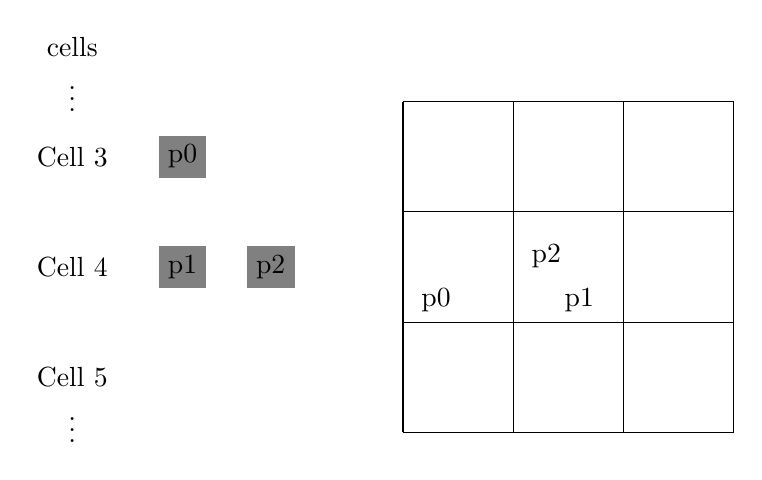
\begin{tikzpicture}
		%define constants
		\def\offGrid{3}
		\def\offP{2.5}
		\def\arrowStart{0.6}
		\def\arrowEnd{1.9}
		
		\def\scale{1.4}
		
		%draw grid scetch
		\foreach \k in {0,...,3} {
			\draw (\scale*\offGrid+\scale*\k,\scale*0)--(\scale*\offGrid+\scale*\k,\scale*3);
			\draw (\scale*\offGrid +\scale*0,\scale*\k)--(\scale*\offGrid+\scale*3,\scale*\k);
		}
		
		\node[] at (\scale*\offGrid+\scale*0.3, \scale*1.2) {p0};
		\node[] at (\scale*\offGrid+\scale*1.6, \scale*1.2) {p1};
		\node[] at (\scale*\offGrid+\scale*1.3, \scale*1.6) {p2};
		
		%draw datastructure scetch
		
		%cells
		\node[] at (\scale*0, +\scale*3.5) {cells};
		
		\node[] at (\scale*0, \scale*2.6 + \scale*0.5) {\vdots};
		
		\node[] at (\scale*0, \scale*2 + \scale*0.5) {Cell 3};
		\node[fill=gray] at (\scale*1, \scale*2+\scale*0.5-\scale*0) {p0};
		
		\node[] at (\scale*0, \scale*1 + \scale*0.5) {Cell 4};
		\node[fill=gray] at (\scale*1, \scale*2+\scale*0.5-\scale*1) {p1};
		\node[fill=gray] at (\scale*1.8, \scale*2+\scale*0.5-\scale*1) {p2};
		
		\node[] at (\scale*0, \scale*0 + \scale*0.5) {Cell 5};
		\node[] at (\scale*0, \scale*-0.4 + \scale*0.5) {\vdots};
	
		
	\end{tikzpicture}
\end{frame}

\begin{frame}
\frametitle{The Cell Data Structure - Approach 3}
	\large
	Idea:
	\vspace{-0.5cm}
	\begin{itemize}
		\item Each Cell only keeps references to their members
		\item No sorting or copying of entire particles required
	\end{itemize} 
	
	%\resizebox{0.5\textwidth }{0.5\textheight }{
		\begin{tikzpicture}
			%define constants
			\def\offGrid{3.5}
			\def\offP{2.5}
			\def\arrowStart{0.6}
			\def\arrowEnd{1.9}
			
			\def\scale{1.4}
			
			%draw grid scetch
			\foreach \k in {0,...,3} {
				\draw (\scale*\offGrid+\scale*\k,\scale*0)--(\scale*\offGrid+\scale*\k,\scale*3);
				\draw (\scale*\offGrid +\scale*0,\scale*\k)--(\scale*\offGrid+\scale*3,\scale*\k);
			}
			
			\node[] at (\scale*\offGrid+\scale*0.3, \scale*1.2) {p0};
			\node[] at (\scale*\offGrid+\scale*1.6, \scale*1.2) {p1};
			\node[] at (\scale*\offGrid+\scale*1.3, \scale*1.6) {p2};
			
			%draw datastructure scetch
			
			%particle vector
			\foreach \k in {0,...,2} {
				\node[fill=gray] at (\scale*\offP, \scale*2+\scale*0.5-\scale*\k) {p$\k$};
			}
			%\node at (\scale*\offP, -\scale*0.6) {particles.end()};
			
			\node[] at (\scale*\offP, +\scale*3.5) {particles};
			
			%cells
			\node[] at (\scale*0, +\scale*3.5) {cells};
			
			\node[] at (\scale*0, \scale*2.6 + \scale*0.5) {\vdots};
			\node[] at (\scale*0, \scale*2 + \scale*0.5) {Cell 3};
			\node[] at (\scale*0, \scale*1 + \scale*0.5) {Cell 4};
			\node[] at (\scale*0, \scale*0 + \scale*0.5) {Cell 5};
			\node[] at (\scale*0, \scale*-0.4 + \scale*0.5) {\vdots};
			
			%arrows
			\draw[-triangle 60] (\scale*\arrowStart, \scale*2 + \scale*0.5) -- (\scale*\arrowEnd, \scale*2 + \scale*0.5);
			
			\draw[-triangle 60] (\scale*\arrowStart, \scale*1 + \scale*0.5) -- (\scale*\arrowEnd, \scale*1 + \scale*0.5);
			
			\draw[-triangle 60](\scale*\arrowStart, \scale*1 + \scale*0.5) -- (\scale*\arrowEnd, + \scale*0.5);
			
			%\draw[-triangle 60] (\scale*\arrowStart, \scale*0 + \scale*0.5) -- (\scale*\arrowEnd, -\scale*0.8 + \scale*0.5);
			
		\end{tikzpicture}
	
\end{frame}

\begin{frame}
	\frametitle{Approach Comparison}
	\large
	\setlength\tabcolsep{0.5cm}
	\def\arraystretch{1.5}
	\begin{tabularx}{\linewidth}{>{\hsize=.33\hsize}X|>{\hsize=.33\hsize}X|>{\hsize=.33\hsize}X}		
		
		Approach 1 & Approach 2 & Approach 3 \\
		\hline
		\textcolor{black}{$+$ Easy to implement} & 
		\textcolor{black}{$+$ Easy to implement} &
		\textcolor{black}{$+$ Easy to implement} \\ 
		
		
		
		\textcolor{black}{$+$ Interface for old Assignments remains unchanged} & 
		\textcolor{black}{$+$ New Implementation of some methods needed} &
		\textcolor{black}{$-$ Interface for old Assignments remains unchanged} \\
		
		\textcolor{black}{$-$ Expensive struct swaps during sorting} & 
		\textcolor{black}{$-$ Expensive struct copies with potential reallocs needed} &
		\textcolor{black}{$+$ References are cheap} \\
		
		\textcolor{black}{$+$ Direct access to particles for calculations} & 
		\textcolor{black}{$+$ Direct access to particles for calculations}&
		\textcolor{black}{$+$ Dereferencing needed} \\		
	\end{tabularx}

	\pause
	\vspace{0.4cm}
	In the end we decided to implement approach 3.
\end{frame}


\begin{frame}[fragile]
	\frametitle{ParticleContainer's new methods}
	\vspace{0.4cm}
	
	\begin{lstlisting}[language=C++]
class ParticleContainer{
	...

	void forAllPairsInSameCell(void (*fun) (Particle& p1, Particle& p1));
	
	void forAllPairsInNeighbouringCell(void (*fun) (Particle& p1, Particle& p1));
	
	void forAllCells(void (*fun)(...));
	
	void forAllDistinctNeighbouringCells(void (*fun) (...));
		
	...
}
\end{lstlisting}

	\large

\begin{itemize}
	\item Functionality of first two methods is sufficient but hard to optimize
	\item Functionality of last two methods results in higher cohesion, but potential for runtime improvement
\end{itemize}
	
\end{frame}

\begin{frame}
	\frametitle{Runtime measurement setup}
	\vspace{2.3cm}
		\large
		\begin{itemize}
			\setlength\itemsep{1em}
			\item<1-> Particles initiated in a square with varying dimensions
			\item<2-> Space between square and domain border kept at 10
			\item<3-> $r_{cutoff} = $const. (aswell as other variables like eps, sig, brown, etc.)
			\item<4-> exact commands to recreate the results are in README and at the end of this presentation
		\end{itemize}
		
\end{frame}


\begin{frame}[fragile]
	\frametitle{Runtime Comparison of different algorithms}
	\begin{columns}
		\column{0.6\linewidth}
			\vspace{-0.9cm}
			\begin{figure}
				\centering
				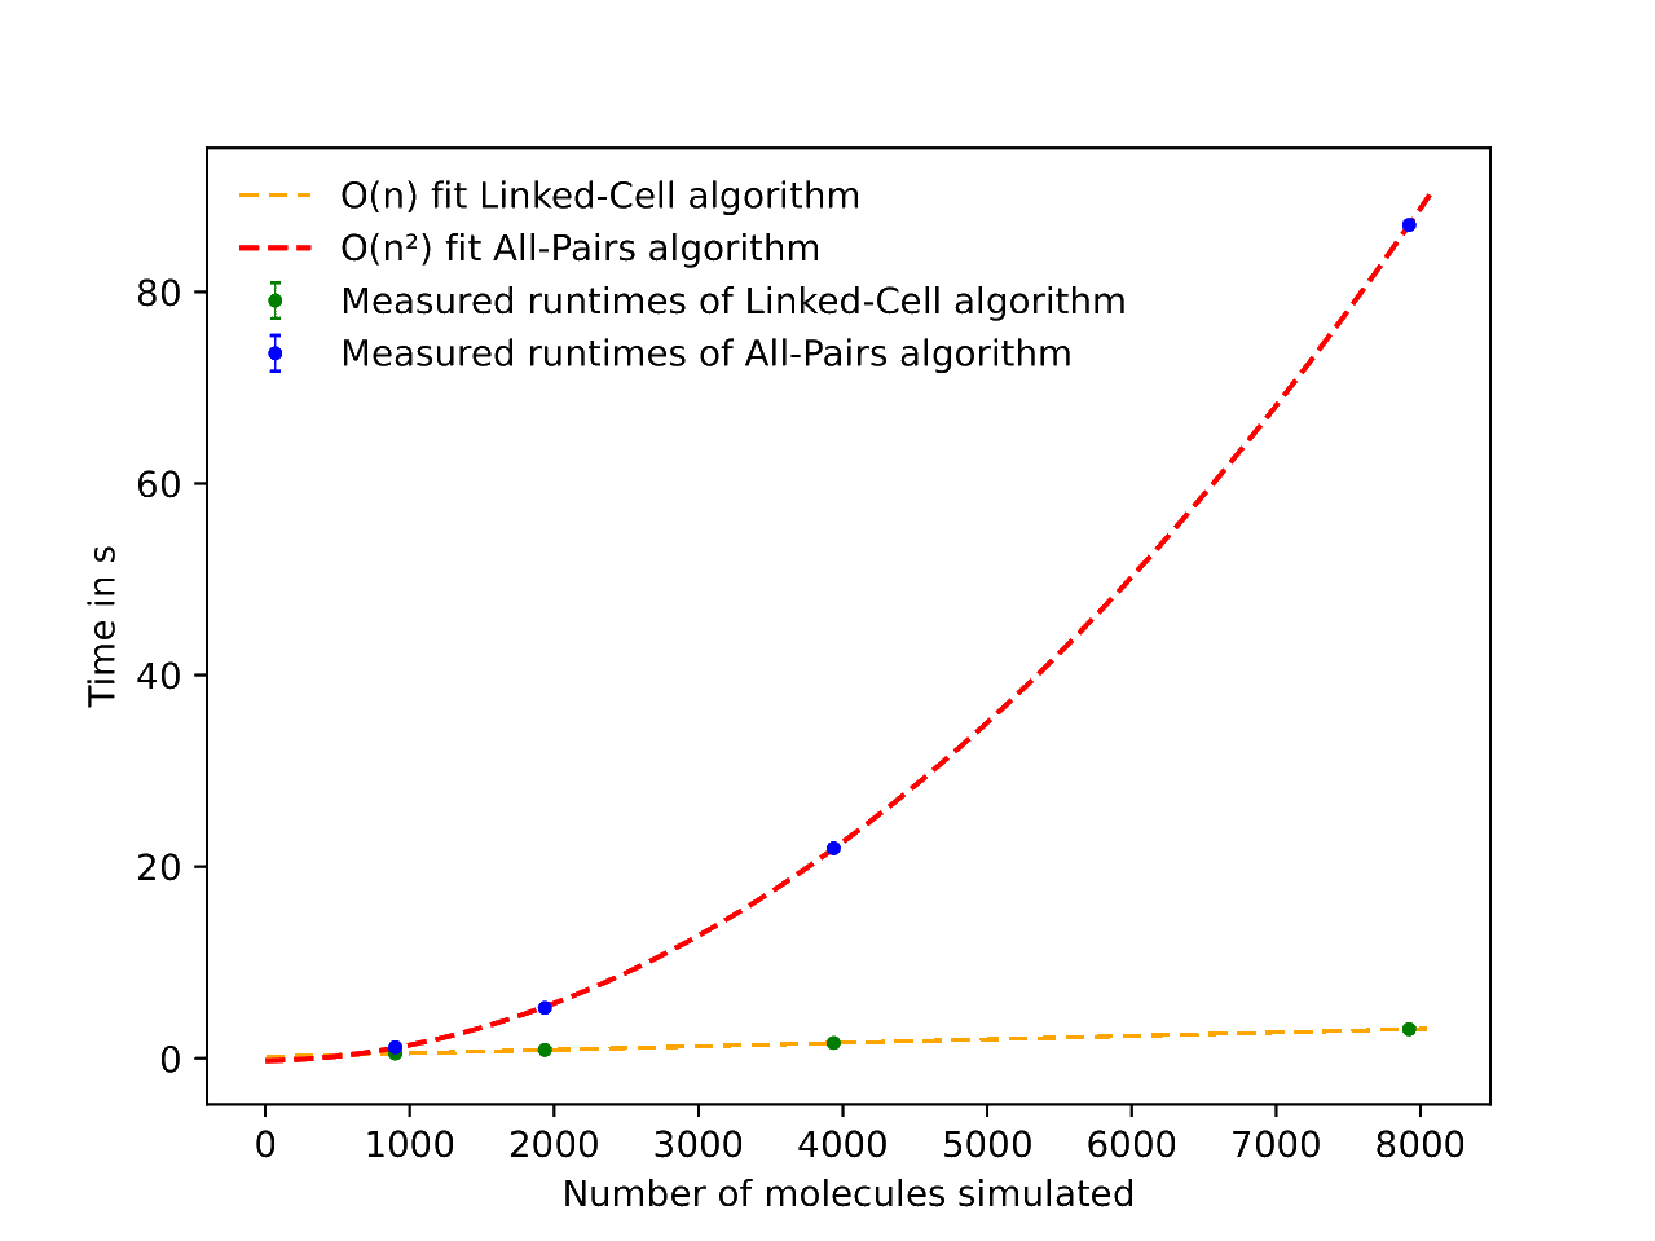
\includegraphics[width=\linewidth]{plot}
				\label{fig:plot}
			\end{figure}
		\column{0.28\linewidth}
		\\
		
		
		\large
		Hardware details:
		\begin{lstlisting}
Ubunutu 20.04 LTS
i7-12700KF @5,0GHz
64GB RAM @ 3200MHz
		\end{lstlisting}
	
	
	\end{columns}
\end{frame}

\begin{frame}{Our Simulation}
	\begin{figure}[h!]
		\centering    
		\movie[label=show3,width=0.7\textwidth,poster
		,autostart,showcontrols,loop] 
		{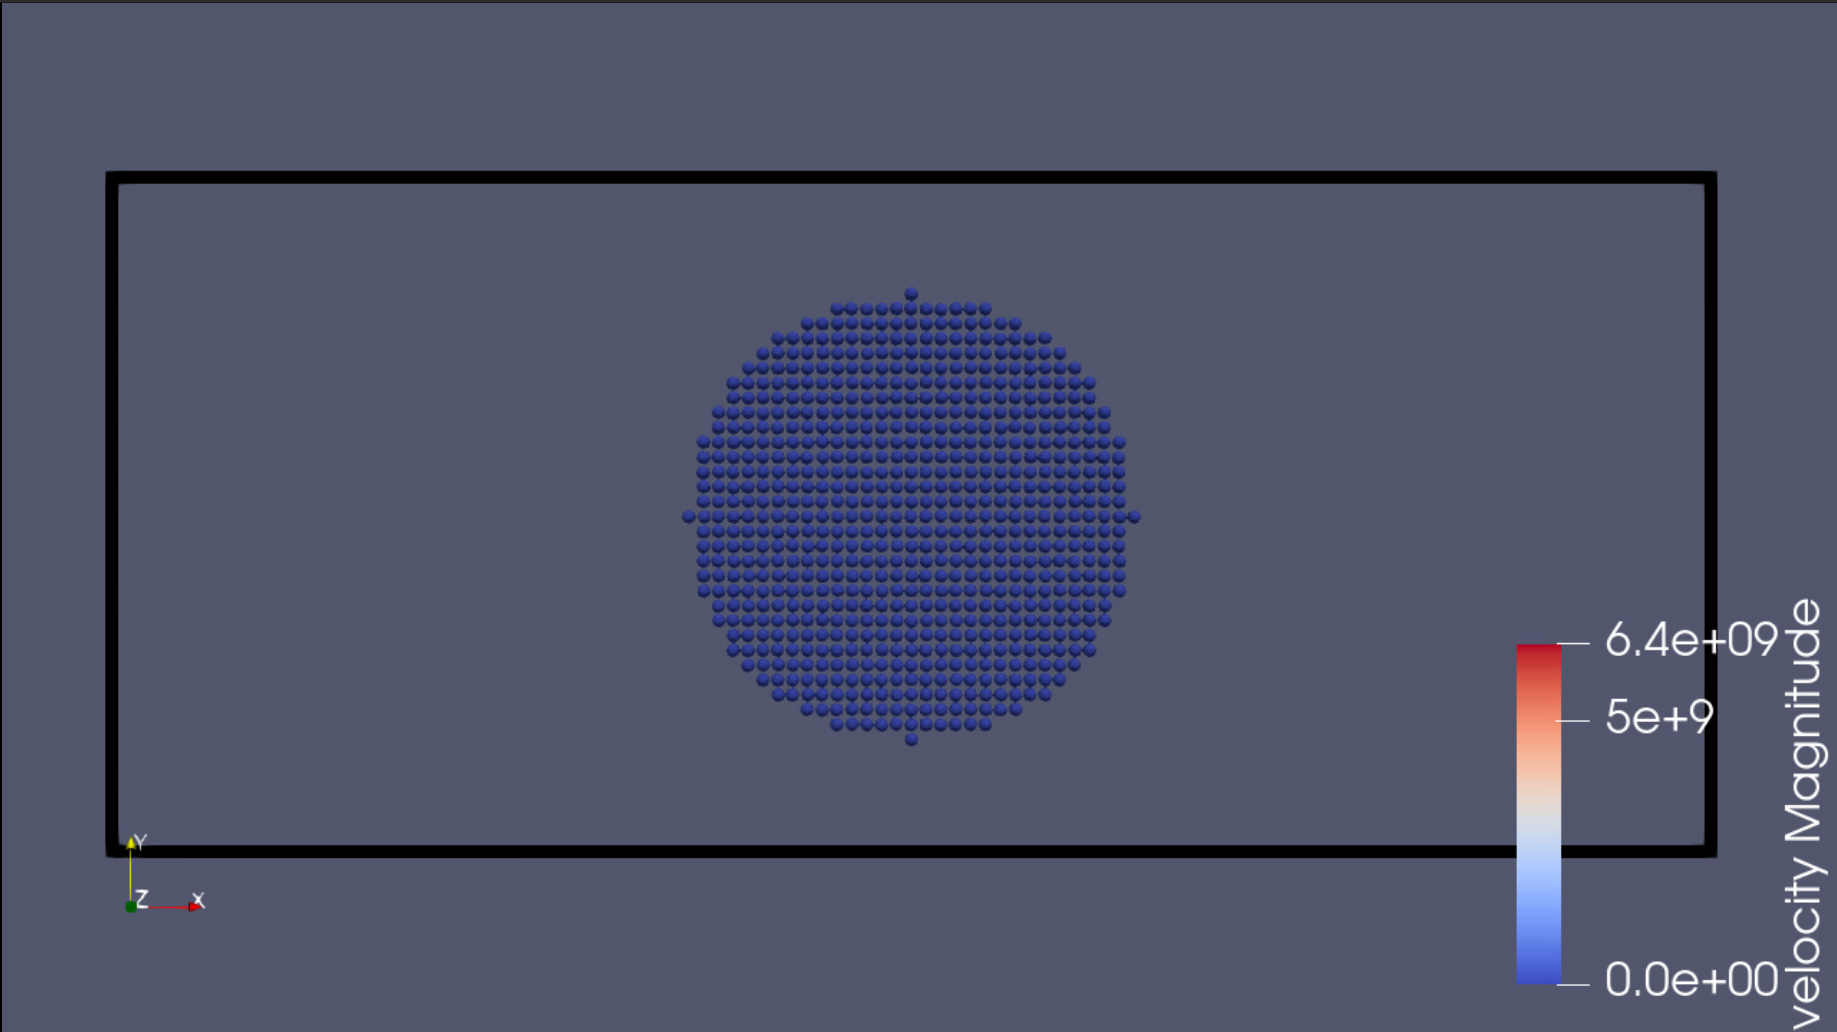
\includegraphics[width=0.7\textwidth]{waterdrop.png}}{drop_dt0-001.mp4}
		%\caption{caption}
	\end{figure} 
\end{frame}

\begin{frame}{Doubling $\Delta t$}
	\begin{figure}[h!]
		\centering    
		\movie[label=show3,width=0.7\textwidth,poster
		,autostart,showcontrols,loop] 
		{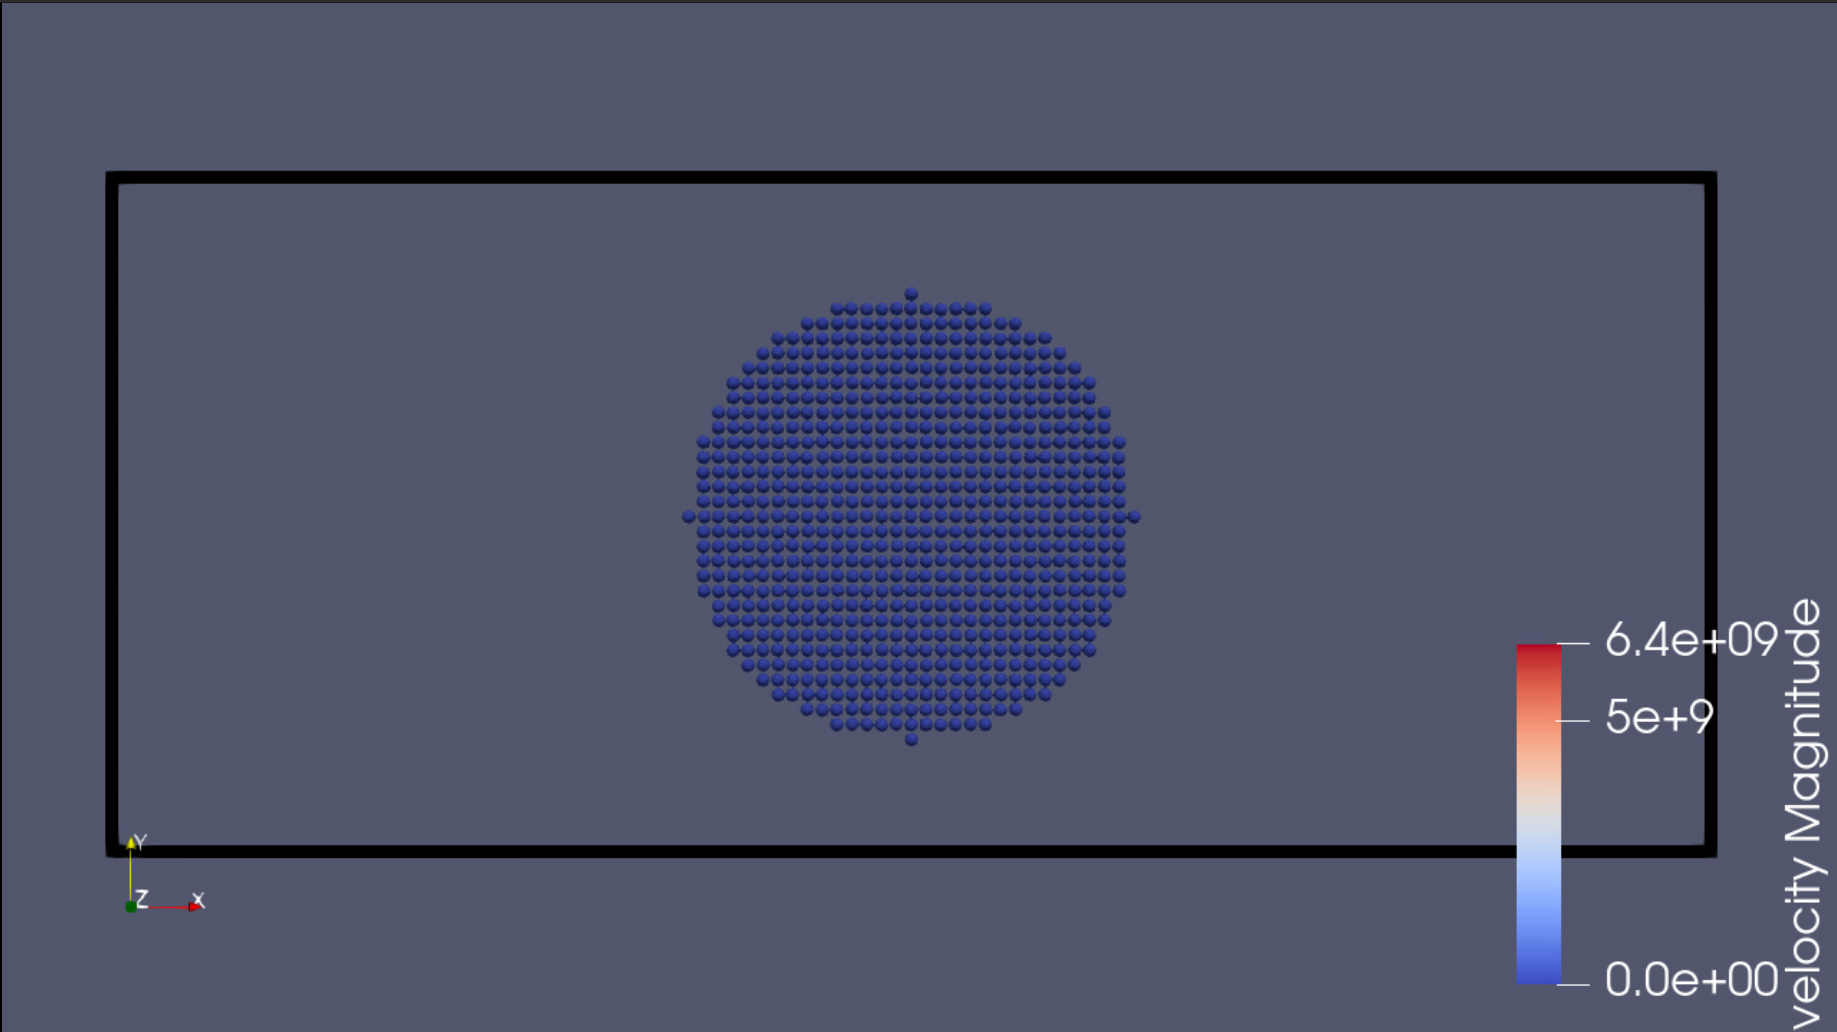
\includegraphics[width=0.7\textwidth]{waterdrop.png}}{drop_dt0-002.mp4}
		%\caption{caption}
	\end{figure} 
\end{frame}

\begin{frame}
	\frametitle{Roadblocks and lessons learned}
	\large
	\begin{itemize}
		\item Play the objective!
		\item Getting together and figuring out an elegant solution for one hour is an hour well spent
		\item Clearly define Interfaces
	\end{itemize}
\end{frame}

\begin{frame}
	\PraesentationBildUhrenturm
	%\PraesentationStartseiteFlaggen
\end{frame}

\begin{frame}
	\frametitle{Recreating benchmarks}
	\large
	Setup and compilation:
	\vspace{-0.7cm}
	\begin{enumerate}
		\item mkdir build output
		\item cd build
		\item cmake ..
		\item make
	\end{enumerate}
	\vspace{-0.6cm}

	Example of bechmark commands:\\
	Linked-Cell algorithm:\\
	./MolSim ../input/square1.txt -dt 0.0005 -et 0.5 -lc 1 -bbox0 50.0 -bbox1 50.0 -f lennardjonescell -rc 3.0 -bench file -i 10 > ../output/lc\_square1.txt
	
	All-Pairs algorithm:\\
	./MolSim ../input/square1.txt -dt 0.0005 -et 0.5 -lc 0 -bbox0 50.0 -bbox1 50.0 -f lennardjones -rc 3.0 -bench file -i 10 > ../output/ap\_square1.txt\\
	
	\large


\end{frame}

\begin{frame}
	\frametitle{Recreating benchmarks}
	\vspace{2.5cm}
	\large
	\begin{itemize}
	\item Results can be found in output-folder
	\item New benchmark files can be written and executed easily
	\item for other testsizes change input file, output file and bbox-size accordingly
	\end{itemize}

	bbox-sizes needed: (50,50), (64,64), (83,83), (109,109)
	
\end{frame}

%\frame[label=blah]{
%	\begin{center}%
%		\href{run:/usr/local/bin/mplayer -fs standard-benchmark.mp4}{
%		\includegraphics[scale=0.25]
%		{Assignment2_Presentation.pdf}}

%		\includemovie{.85\textheight}{.85\textheight}{standard-benchmark.mp4}%
%	\end{center}%
%	\note{%
%		\begin{itemize}
%			\item blah
%			\item blah
%		\end{itemize}
%	}%
%}


%%%%%%%%%%%%%%%%%%%%%%%%%%%%%%%%%%%%%%%%%%%%%%%%%%%%%
%% Folie: Gültigkeit der Masterfolien              %%
%%%%%%%%%%%%%%%%%%%%%%%%%%%%%%%%%%%%%%%%%%%%%%%%%%%%%
